\documentclass[crop,tikz]{standalone}

\usepackage{pgfplots}
\tikzset{>=latex}

\pgfplotsset{
  inverted/.style = {
    every axis legend/.append style={
      draw=white,
      fill=hardblack,
      text=white
    }
  }
}

\begin{document}
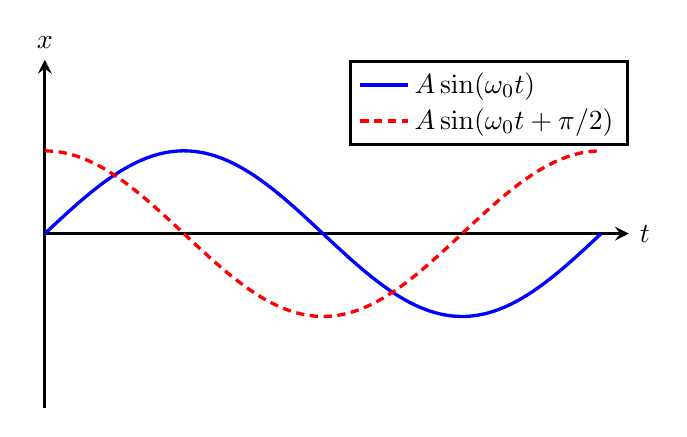
\begin{tikzpicture}
\begin{axis}[
  very thick,
  width=9cm,
  height=6cm,
  domain={0}:{2*pi},
  samples=50,
  axis y line=middle,
  axis x line=middle,
  xlabel={$t$},
  ylabel={$x$},
  xlabel style={right},
  ylabel style={above},
  xmin=0, xmax={2.1*pi},
  ymin=-2.1, ymax=2.1,
  xtick={\empty},
  xticklabels={\empty},
  ytick={\empty},
  yticklabels={\empty},
  legend cell align={left},
  legend style={at={(1,1)},anchor=north east}
  ]
  \addplot[blue,smooth] { sin(deg(x)) };
  \addlegendentry{$A\sin(\omega_0 t)$};
  \addplot[red,smooth,densely dashed] { sin(deg(x+pi/2)) };
  \addlegendentry{$A\sin(\omega_0 t + \pi/2)$};
\end{axis}
\end{tikzpicture}
\end{document}
